% =========================================================================== %

\begin{frame}[t,plain]
\titlepage
\end{frame}

% =========================================================================== %

\begin{frame}{About Me}
%
\begin{columns}
\column{.5\linewidth}
\begin{itemize}
\item Former Student of UR
	\begin{itemize}
	\item 2015-2021: Physics
	\item 2020-2022: Computational Science
	\item Have been involved in UR IT courses since 2018
	\end{itemize}
\item Now: Software Development Engineer
\item Hobby Enthusiast
	\begin{itemize}
	\item First Programming Language (BASIC) when I was 9 years old
	\item So a little over 20 years of semi-professional busying myself with computers
	\item I like sharing nerdy stuff in spite of my limited time
	\end{itemize}
\end{itemize}
%
\column{.5\linewidth}
\begin{itemize}
\item Human Languages
	\begin{itemize}
	\item German
	\item English
	\item French
	\end{itemize}
\item Computer Languages
	\begin{itemize}
	\item Python
	\item C, C++
	\item Java, Groovy
	\item BASIC (VisualBASIC, freeBASIC, QBASIC)
	\item \LaTeX
	\item (some Assembly, Bash Shell Scripting, Julia; even less HTML, CSS, PowerShell, MS-DOS Batch, MySQL, Maple, Matlab)
	\end{itemize}
\end{itemize}
\end{columns}
%
\end{frame}

% =========================================================================== %

\begin{frame}{About this Course}
%
\begin{itemize}
\item Classic presentation plus workshop-like open discussion
\item No exercises, no grades, no mandatory attendence -- this is a hobby project of mine
\item I prepared a choice of topics ...
\item ... but want to adapt to your needs
\item So interaction/feedback is greatly appreciated
	\begin{itemize}
	\item Preferably direct
	\item Also: Email (\todo{put my email address here})
	\end{itemize}
\item All media (codes, slides, ...) provided online
	\begin{itemize}
	\item See GRIPS: \todo{GRIPS link}
	\item \todo{how to find without link}
	\end{itemize}
\item Scope: Whatever is interesting for a majority of you
\end{itemize}
%
\end{frame}

% =========================================================================== %

\begin{frame}{Course Environment}
%
\begin{itemize}
\item You should have installed ...
	\begin{itemize}
	\item A Python 3 interpreter
		\begin{itemize}
		\item Preferably newest version (currently Python 3.10)
		\item Older versions usually work just as well, but some minor details might have changed, or features might not be available
		\item Check on the command line: \texttt{python3 --version}
		\end{itemize}
	\item A means to install Python packages
		\begin{itemize}
		\item E.\;g. \texttt{pip}, \texttt{conda}, \texttt{venv}, ...
		\item Just ask me after the presentation if you are unsure
		\end{itemize}
	\item Packages \texttt{numpy} and \texttt{matplotlib}
	\item Some IDE
		\begin{itemize}
		\item \textbf{PyCharm} (Community Edition) -- my recommendation\\
			Many features (debugger, refactory, integration of unit tests, connection to git, ...)
		\item \textbf{Spyder 4} -- from the UR courses Introduction to Python\\
			Still some cool featuers, lacks refactory options, but good one-stop-solution with Anaconda
		\item \textbf{Notepad++/Kate/geany plus command line} -- for minimalists\\
			Gets the job done, but you'll have to do everything by hand
		\end{itemize}
	\end{itemize}
\end{itemize}
%
\end{frame}

% =========================================================================== %

\begin{frame}{The First Few Sessions (Recommendation)}
%
\begin{itemize}
\item Today
	\begin{itemize}
	\item Project Structure: Classes and Modules
	\item Discussing example simulation: non-interacting particles in a potential
	\end{itemize}
\item Next time
	\begin{itemize}
	\item Discussing efficiency -- Big O Notation
	\item How numpy makes Python fast (by not being Python)
	\end{itemize}
\item Later On
	\begin{itemize}
	\item SciPy: Integration, Fourier Analysis, Curve Fitting, ODEs and PDEs
	\item Python Concepts: Iterators, Decorators, Magic Methods, Type Annotations
	\item IT Concepts: Unit Tests, Git Repositories, Automated Documentation
	\item Pandas -- Queries on data frames
	\item Parallelization -- using multiple processors at once
	\item ...
	\end{itemize}
\end{itemize}
%
\begin{center}
\emph{... unless you ask me to do something else}
\end{center}
%
\end{frame}

% =========================================================================== %

\begin{frame}{Setting Up A Project}
%
\begin{columns}
\column{.6\linewidth}
\begin{itemize}
\item Humans have a \emph{top down} approach of thinking
	\begin{itemize}
	\item Web of relationships
	\item Hierarchical organization
	\item Allows to reduce mental load (thinking about lower level items only implied)
	\end{itemize}
\item Computers need to implement a \emph{bottom up} approach
	\begin{itemize}
	\item All variables in memory
	\item Result emerges from interaction of these components
	\end{itemize}
\item Coder must manage both
	\begin{itemize}
	\item Naive approach: think like a machine. High mental load, error prone
	\item Better: mirror human like thinking patterns!
	\end{itemize}
\end{itemize}
%
\column{.4\linewidth}
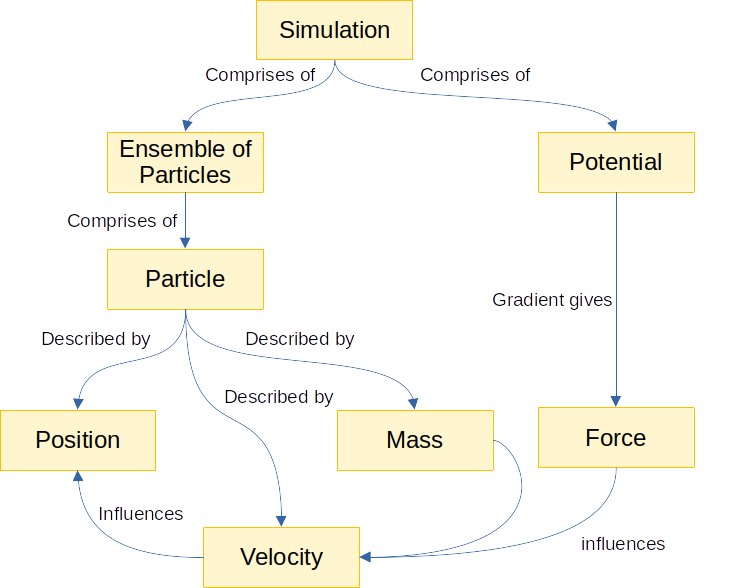
\includegraphics[width=\linewidth]{./gfx/01-structure}
\end{columns}
%
\end{frame}

% =========================================================================== %

\begin{frame}{Classes: Representing Data in Context}
%
\begin{itemize}
\item Remember: \inPy{class}es are data collections plus predefined interactions with the grouped data
\item Essentially: fancy \inPy{dict}s
\item Allows to separate/abstract away \emph{intent} from \emph{implementation}
	\begin{itemize}
	\item Intent: Method names, \zB \texttt{Potential.getForce(coordinates)}
	\item Implementation: How is the potential stored in the first place? What data types do I use? Runtime concerns; Failsafes; ...
	\end{itemize}
\item Write \emph{interfaces} first, then go about implementing them
	\begin{itemize}
	\item Interface: Just the method names without any code behind
	\item \inPy{def getForce(coordinates) : pass}
	\item One class for each \emph{sufficiently complex concept} your system features
	\item \emph{Sufficiently complex concept}: Up to debate and personal taste
	\item Rule of thumb: anything which I can ask more questions than \emph{what are your atoms}?
	\end{itemize}
\end{itemize}
%
\end{frame}

% =========================================================================== %

\begin{frame}{Wrapper classes}
%
Example \inPy{class Particle}:
\begin{itemize}
\item Essentially: group of 5 real numbers (2D case)
	\begin{itemize}
	\item x- and y-position
	\item x- and y-velocity
	\item mass
	\item[\Thus] can (and should) be grouped in one numpy-array
	\end{itemize}
\item But: Readability! Compare ...
	\begin{itemize}
	\item \texttt{particle[0:2]}
	\item \texttt{particle.get\_position()}
	\item \texttt{particle["position"]}
	\end{itemize}
\item And: Custom operations! Compare
	\begin{itemize}
	\item \texttt{particle[0:4] += velocity\_and\_acceleration * dt}
	\item \texttt{particle += velocity\_and\_acceleration * dt}
	\end{itemize}
\item[\Thus] Code should only be concerned with one layer of the problem at hand!
\end{itemize}
%
\end{frame}

% =========================================================================== %

\begin{frame}{Generic Code vs. Specialized Code}
%
\begin{itemize}
\item Example: Number of dimensions
\item Degrees of freedom propagage through your system
	\begin{itemize}
	\item[\Thus] More mental load, more that can break
	\item Often unforseen side effects
		\begin{itemize}
		\item E.\;g.: Increases complexity of computing force field
		\end{itemize}
	\end{itemize}
\item (Potentially) icreases complexity in use (need to specify the special case each time used. Can sometimes be deduced or taken from default values)
\item Advantage in reusability
	\begin{itemize}
	\item May be known from the overall scope of the project
	\item May come unforseen. More often on function/method level than on class level
	\end{itemize}
\item[\Thus] Generalize only if necessary or \emph{very easy}
	\begin{itemize}
	\item Rewriting a \emph{correctly working} piece of code is often difficult enough
	\item Failsafe/easy to use code is worth more than generic code
	\end{itemize}
\end{itemize}
%
\end{frame}

% =========================================================================== %

\begin{frame}{Classes: Order of implementation}
%
\begin{itemize}
\item (Begin with the interface, maybe only on paper)
\item Write the \inPy{__init__} first
	\begin{itemize}
	\item Which attributes do describe your object?
	\item Which data type and grouping is best suited for this task?
	\item Parameters to the constructor. Again, need not mirror the inner structure.
	\item Example: \texttt{Particle(position, velocity, mass)} (3 parameters). Internally represented by one member (\texttt{data}), which stores five numbers
	\item Thik about default parameters and validity checks
		\begin{itemize}
		\item What if a user accidentally provides a string for either of them?\\
			Usually, just \inPy{raise} an Exception \emph{with meaningful text}
		\item Do I always need to provide all five numbers? Maybe allow \emph{null-initialization}
		\end{itemize}
	\end{itemize}
\item Then: \inPy{__str__}
	\begin{itemize}
	\item Greatly facilitates debugging when you only \texttt{print(particle)} to see \texttt{Particle at [4.20, 3.14], velocity = [0.00, 0.00], mass = 1.00}
	\end{itemize}
\end{itemize}
%
\end{frame}

% =========================================================================== %

\begin{frame}{Classes: Order of implementation}
%
\begin{itemize}
\item Classes themselves: bottom up
\item I.\;e. the "atomic" classes (the elements of composed systems first
\item If mutual interdependence (A affects B, and B affects A; neither is \enquote{element of} the other):
	\begin{itemize}
	\item Avoid if possible, \zB via return values
	\item Start with whichever is easier on your head
	\item Usually the one with fewer active side interactions
	\end{itemize}
\item Building Software bottom up allows to parallelly test the code
	\begin{itemize}
	\item Unittests: Separate program that instantiate your class and use all the methods
	\item Pass if expected results produced
	\item Python offers a number of unittest systems \Thus another evening
	\end{itemize}
\end{itemize}
%
\end{frame}